%versi 2 (8-10-2016) 
\chapter{Pendahuluan}
\label{chap:intro}
   
\section{Latar Belakang}
\label{sec:label}
Perangkat lunak KIRI\footnote{\url{https://projectkiri.id/} (diakses 14 Februari 2025)} (lihat Gambar \ref{fig:kiri}) adalah perangkat lunak berbasis \textit{web} yang dirancang untuk membantu pengguna menemukan rute perjalanan ketika menggunakan angkot untuk di Bandung serta TransJakarta dan Commuterline untuk di DKI Jakarta. Pada perangkat lunak KIRI, pengguna dapat memasukkan titik awal perjalanan dan titik tujuan. KIRI kemudian akan mencarikan berbagai alternatif rute yang bisa digunakan untuk mencapai tujuan tersebut.
\begin{figure}[h] 
	\centering  
	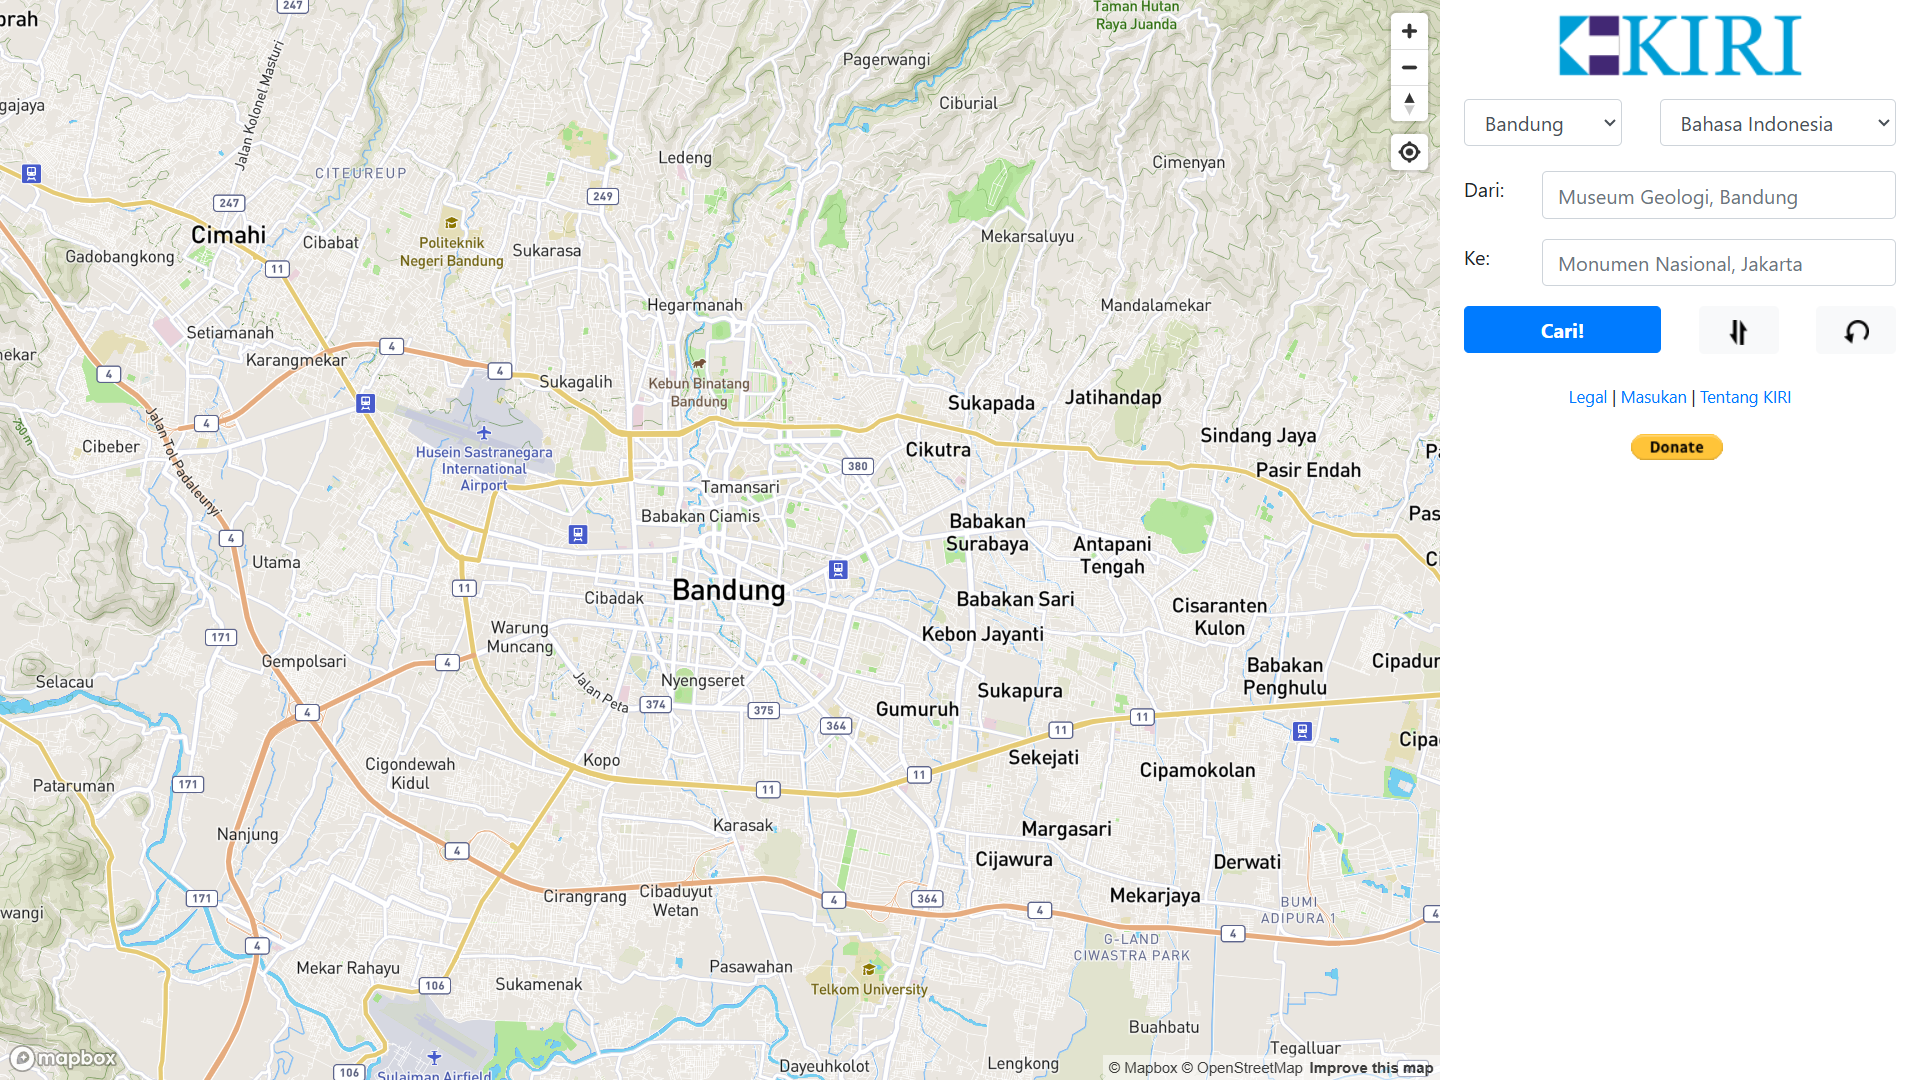
\includegraphics[width=1\textwidth]{KIRI.png}  
	\caption{Tampilan halaman perangkat lunak KIRI}
	\label{fig:kiri} 
\end{figure}
\\
KIRI akan memberikan informasi mengenai langkah-langkah yang harus ditempuh oleh pengguna yang akan bepergian dari suatu tempat ke tempat tujuannya, mulai dari seberapa jauh pengguna harus berjalan untuk menaiki angkot yang bersangkutan, di mana pengguna harus naik atau turun angkot tersebut, seberapa jauh lagi pengguna harus berjalan sampai ke lokasi tujuan, dan seberapa lama estimasi waktu perjalanan yang akan ditempuh (lihat Gambar \ref{fig:kiri2}).
\begin{figure}[H] 
	\centering  
	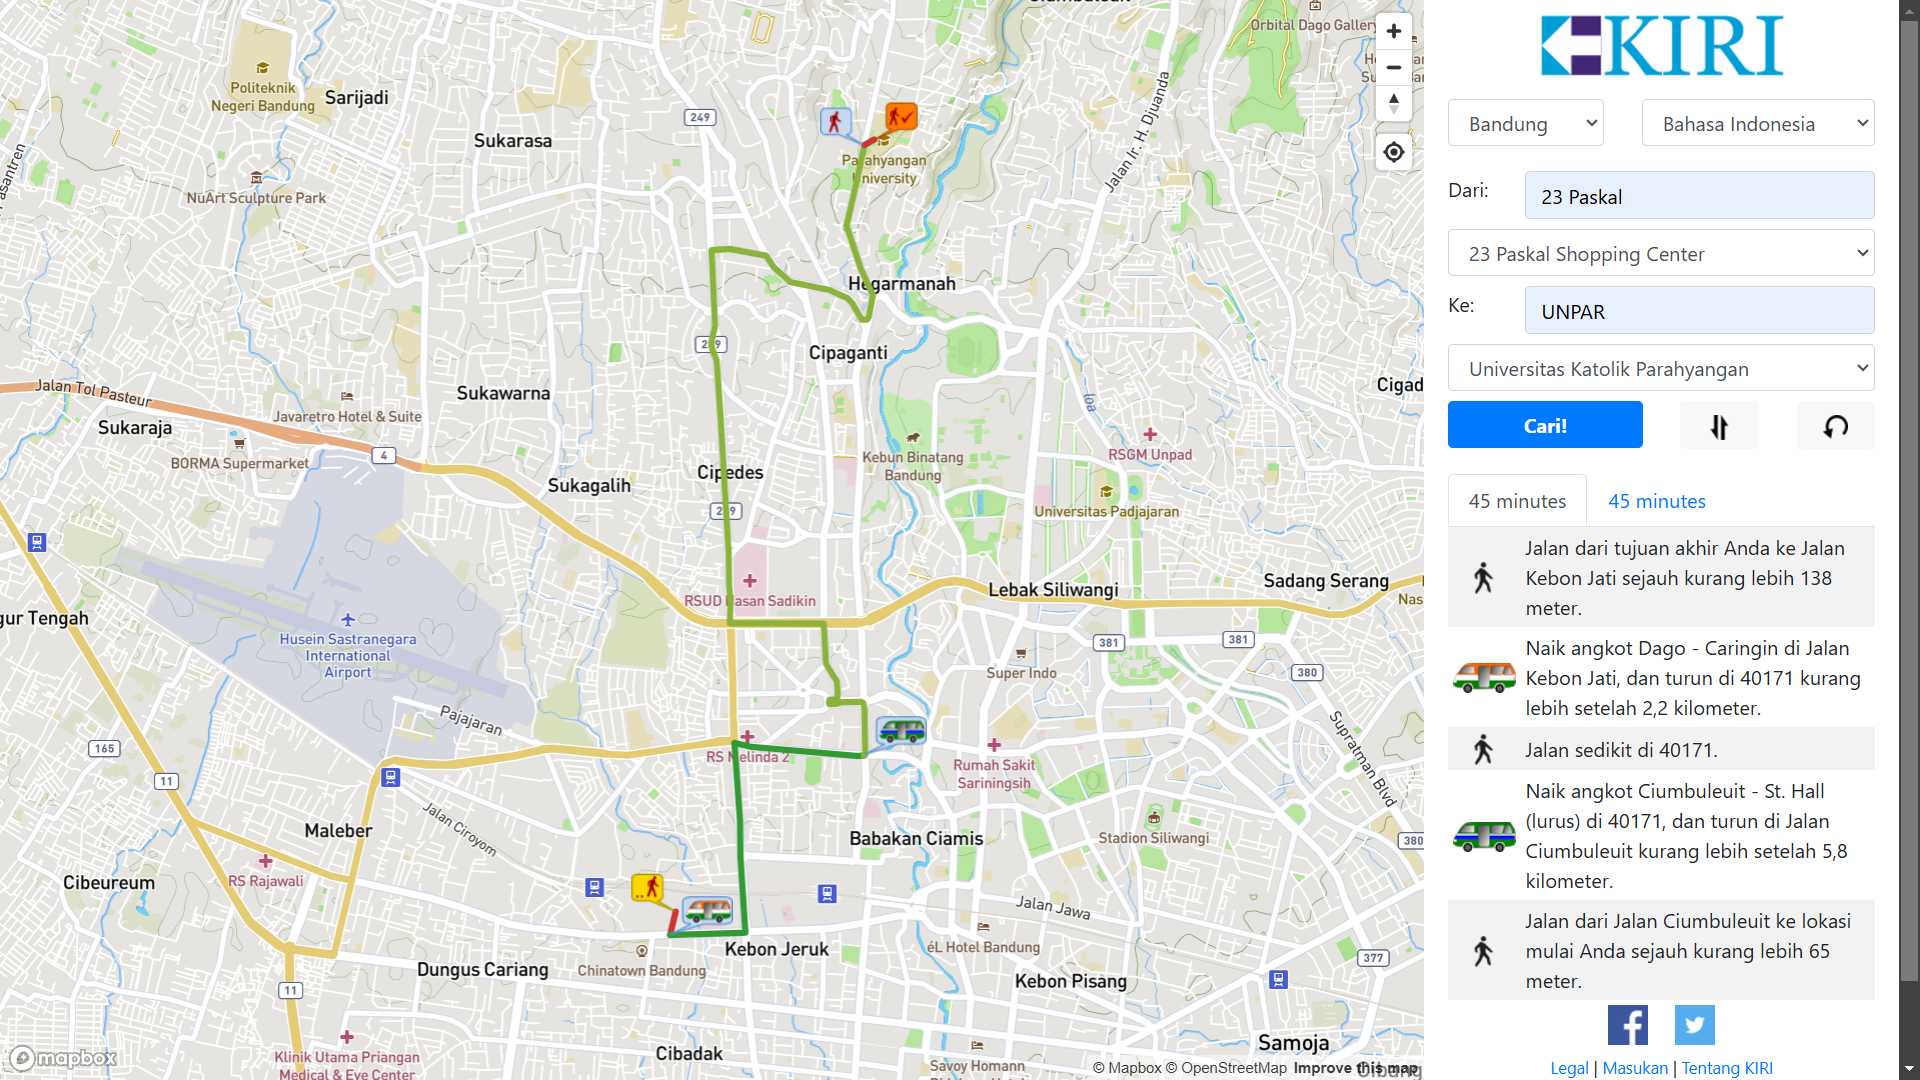
\includegraphics[width=1\textwidth]{KIRI-2.png}  
	\caption{Tampilan perangkat lunak KIRI, setelah menerima masukan}
	\label{fig:kiri2} 
\end{figure}
\noindent
Arsitektur aplikasi KIRI terbagi menjadi dua bagian utama. Bagian \textit{frontend}, yang dinamakan Tirtayasa dan dibangun menggunakan bahasa pemrograman PHP serta mengandalkan basis data MySQL untuk menyimpan serta mengelola data. Selain itu, Tirtayasa juga menggunakan framework CodeIgniter 3. Saat menerima permintaan pencarian, Tirtayasa meneruskannya ke bagian \textit{backend}, yaitu NewMenjangan. Hasil dari NewMenjangan kemudian diformat agar dapat dibaca dengan baik oleh pengguna. Bagian ini diimplementasikan dalam bahasa pemrograman Java dan berperan penting dalam perhitungan rute optimal.~\cite{nugroho_natali:17:KIRI}
\\
NewMenjangan merupakan program \textit{daemon} yang berjalan secara otomatis saat server dinyalakan dan terus beroperasi hingga server dimatikan. \textit{Daemon} sendiri adalah program komputer yang berjalan dilatar belakang dan tidak berinteraksi langsung dengan pengguna\footnote{\url{https://www.ibm.com/docs/en/aix/7.1?topic=processes-} (diakses 14 Februari 2025)}. Pada saat eksekusi, NewMenjangan terhubung ke basis data MySQL untuk mengambil data rute angkot yang tersimpan dalam format LineString. LineString adalah salah satu tipe data geometris dalam MySQL yang mewakili satu atau lebih segmen garis yang terhubung. LineString terdiri dari urutan titik (\textit{point}) yang membentuk jalur atau lintasan\footnote{\url{https://dev.mysql.com/doc/refman/8.4/en/gis-linestring-property-functions.html} (diakses 14 Februari 2025)}. Setiap titik pada LineString merepresentasikan lokasi potensial untuk penumpang naik atau turun. Dari data tersebut, NewMenjangan membangun \textit{weighted graph} dalam memori (RAM) dalam bentuk \textit{adjacency list} dan melakukan prakomputasi. Setiap titik pada LineString menjadi akan \textit{node}, dan antara titik ke-i dan titik ke-(i+1) dihubungkan dengan \textit{edge}. Jika ada dua titik dari rute angkot berbeda yang berdekatan (jarak di bawah konstanta tertentu), maka dibuatkan juga \textit{edge}, yang menunjukkan kemungkinan seseorang dapat turun dari suatu angkot dan naik ke angkot lainnya untuk meneruskan perjalanan. 
\newpage
\noindent
Saat NewMenjangan menerima permintaan pencarian dari titik A ke titik B, kedua titik tersebut dijadikan \textit{node} sementara, dan dibuatkan \textit{edge} sementara ke \textit{node-node} yang sudah ada sebelumnya, jika jaraknya di bawah konstanta tertentu. Pencarian jarak terdekat pada graf tersebut dilakukan menggunakan algoritma Dijkstra versi teroptimasi (\textit{priority queue} dengan struktur data \textit{heap}). Proses ini dapat dilakukan secara paralel dengan aman (\textit{thread-safe}) tanpa mengubah graf utama.
\\
Seperti pada judul tugas akhir ini, akan dilakukan modularisasi algoritma \textit{shortest path} pada perangkat lunak KIRI menggunakan strategy pattern. Modularisasi adalah membagi perangkat lunak menjadi beberapa komponen yang terpisah, yang disebut modul, yang masing-masing dapat diakses dan diberi nama secara independen tetapi bekerja bersama untuk memenuhi kebutuhan sistem~\cite{Pressman:19:Software}. Saat ini algoritma yang digunakan KIRI masih terikat dengan algoritma Dijkstra. Oleh karena itu, pada tugas akhir ini akan diimplementasikan algoritma lainnya, yaitu algoritma A* dan Floyd-Warshall sebagai \textit{concrete strategy}. Selain itu, akan dilakukan juga penerapan arsitektur kelas \textit{strategy pattern} sehingga aplikasi KIRI akan menjadi lebih fleksibel dalam pemilihan algoritma \textit{shortest path} yang akan digunakan dan juga memudahkan apabila akan dilakukan perubahan atau perbaikan pada suatu algoritma yang digunakan.

\section{Rumusan Masalah}
\label{sec:rumusan}
Rumusan masalah berdasarkan latar belakang yang sudah dipaparkan adalah sebagai berikut:
\begin{enumerate}
    \item Bagaimana cara melakukan perubahan kode pada NewMenjangan untuk menerapkan strategy pattern?
    \item Bagaimana mengimplementasikan algoritma A* dan Floyd Warshall sebagai \textit{concrete strategy}?
\end{enumerate}

\section{Tujuan}
\label{sec:tujuan}
Tujuan berdasarkan rumusan masalah yang sudah dipaparkan adalah sebagai berikut:
\begin{enumerate}
    \item Melakukan perubahan arsitektur kelas dengan menerapkan strategy pattern.
    \item Melakukan implementasi algoritma A* dan Floyd Warshall.
\end{enumerate}

\section{Batasan Masalah}
\label{sec:batasan}
Batasan masalah pada tugas akhir ini adalah sebagai berikut:
\begin{enumerate}
    \item Ukuran graf yang sangat besar sehingga untuk algoritma Floyd-Warshall tidak dapat berjalan dengan baik apabila seluruh data digunakan.
\end{enumerate}

\section{Metodologi}
\label{sec:metlit}
Metodologi yang akan digunakan dalam pembuatan tugas akhir ini adalah sebagai berikut:
	\begin{enumerate}
		\item Melakukan eksplorasi fungsi-fungsi dan cara kerja perangkat lunak KIRI.
		\item Mempelajari modul-modul yang terdapat pada Tirtayasa dan NewMenjangan.
		\item Mempelajari bahasa pemrograman PHP dan framework CodeIgniter 3.
		\item Melakukan studi literatur mengenai penerapan arsitektur kelas strategy pattern.
    		\item Mempelajari cara kerja algoritma Dijkstra, A*, dan Floyd Warshall.
    		\item Mengubah implementasi algoritma Dijkstra yang sudah ada ke dalam strategy pattern.
    		\item Mengimplementasikan algoritma A-star dan Floyd Warshall.
    		\item Melakukan pengujian dan eksperimen.
    		\item Menulis dokumen tugas akhir.
	\end{enumerate}

\section{Sistematika Pembahasan}
\label{sec:sispem}
Tugas akhir ini akan disusun menjadi beberapa bab sebagai berikut:
\begin{itemize}
    \item \textbf{Bab 1:} Pendahuluan
    \\ Bab ini berisi latar belakang, rumusan masalah,tujuan, batasan masalah, metodologi, dan sistematika pembahasan.
    \item \textbf{Bab 2:} Landasan Teori
    \\ Bab ini berisi dasar dari teori-teori yang dibutuhkan dalam penelitian ini, seperti KIRI, \textit{Design Pattern} dan \textit{Strategy Pattern}, MySQL, LineString, Graf, dan juga algoritma-algoritma \textit{shortest path} yang akan diimplementasikan, yaitu algoritma Dijkstra, algoritma Floyd-Warshall, dan algoritma A*.
    \item \textbf{Bab 3:} Analisis
    \\ Bab ini berisi analisis dari sistem KIRI saat ini yang belum mengimplementasikan \textit{Strategy Pattern} serta hanya mengimplementasikan algoritma Dijkstra dan juga analisi sistem usulan yang akan mengimplementasikan \textit{Strategy Pattern} serta 2 algoritma \textit{shortest path} lainnya, yaitu algoritma Floyd-Warshall, dan algoritma A*. 
    \item \textbf{Bab 4:} Perancangan
    \\ Bab ini berisi rancangan dari pengembangan yang akan dilakukan perangkat lunak KIRI.
    \item \textbf{Bab 5:} Implementasi dan Pengujian
    \\ Bab ini berisikan pengimplementasian yang akan dilakukan untuk pengembangan perangkat lunak KIRI. Selain itu, bab ini juga berisi pengujian fungsi-fungsi pada perangkat lunak KIRI setelah dilakukan pengembangan.
    \item \textbf{Bab 6:} Kesimpulan dan Saran
    \\ Bab ini berisi kesimpulan dari hasil pengembangan perangkat lunak kiri dan juga saran untuk pengembangan berikutnya.
        
\end{itemize}